\documentclass[11pt,letterpaper]{article}
\usepackage{geometry}\geometry{left=1.5in,right=1.5in,}
\usepackage[utf8]{inputenc}
\usepackage{amsmath}
\usepackage{mathtools}
\usepackage{amsfonts}
\usepackage{amssymb}
\usepackage{graphicx}
\usepackage{caption}
\usepackage{subcaption}
\usepackage{enumerate}
\usepackage{listings}
\usepackage{color}
\usepackage{tikz}


% setup commands
\newcommand{\rank}{\mathrm{rank}}
\newcommand{\innerprod}[2]{\left\langle #1, #2 \right\rangle}
\newcommand{\abs}[1]{\left\lvert #1 \right\rvert}
\newcommand{\norm}[1]{\left\lVert #1 \right\rVert}
\newcommand{\Expect}[1]{{\rm I\kern-.3em E} \left[ #1 \right]}
\newcommand{\Var}[1]{\mathrm{Var} \left( #1 \right)}
\newcommand{\Cov}[1]{\mathrm{Cov} \left( #1 \right)}
\newcommand{\vect}[1]{\begin{bmatrix} #1 \end{bmatrix}}


% setup environment
\newenvironment{proof}{\paragraph{Proof:}}{\hfill$\square$}

\definecolor{codegreen}{RGB}{133,153,0}
\definecolor{codecyan}{RGB}{42,161,152}
\definecolor{codeblue}{RGB}{38,139,210}
\definecolor{base1}{RGB}{147,161,161} % comment
\definecolor{base3}{RGB}{253,246,227} % background
\definecolor{base00}{RGB}{101,123,131} % default code
\definecolor{base01}{RGB}{88,101,117} % optional emphasized content
\lstdefinestyle{codestyle}{
	backgroundcolor=\color{base3},   
	basicstyle=\footnotesize\color{base00},
	numberstyle=\tiny\color{base00},
	commentstyle=\color{base1},
	keywordstyle=\bfseries\color{codegreen},
	stringstyle=\color{codecyan},
	%identifierstyle=\color{codeblue},
	breakatwhitespace=false,         
	breaklines=true,                 
	captionpos=b,                    
	keepspaces=true,                 
	numbers=left,                    
	numbersep=5pt,                  
	showspaces=false,                
	showstringspaces=false,
	showtabs=false,                  
	tabsize=4
}

% information
\author{Khoi-Nguyen Mac}
\title{ECE551 - Homework 3-4}

\begin{document}
	\maketitle
	
	\section{Sampling and Interpolation for Band-Limited Vectors}\label{sec:p1}

\begin{enumerate}[(a)]
\item We have the Fourier vector
\[w_k[n] = e^{j\frac{2\pi k n}{M}}\]
and
\[2\cos x = e^{jx} + e^{-jx}\]
So
\begin{align*}
	x_1[n] 
	&= 1 + \cos\left(\frac{2\pi n}{M}\right) + \cos\left(\frac{8\pi n}{M}\right) \\
	&= w_0[n] + \frac{1}{2}\left(e^{j\frac{2\pi n}{M}} + e^{-j\frac{2 \pi n}{M}}\right) + \frac{1}{2}\left(e^{j\frac{8\pi n}{M}} + e^{-j\frac{8 \pi n}{M}}\right) \\
	&= w_0[n] + \frac{1}{2}\left(w_1[n] + w_{-1}[n] + w_4[n] + w_{-4}[n] \right)
\end{align*}
Its DFT is
\begin{align*}
	X_1[k] 
	&= \sum_{n=0}^{M-1} x_1[n] w_{-k}[n] \\
	&= \frac{1}{2} \left( \sum_{n=0}^{M-1} 2w_{-k}[n] + w_{-k-1}[n] + w_{-k+1}[n] + w_{-k-4}[n] + w_{-k+4}[n]\right)
\end{align*}
We can see that
\begin{align*}
	\sum_{n=0}^{M-1} w_k[n]
	&= \sum_{n=0}^{M-1} \exp\left(j\frac{2 \pi k}{M}\right)^n \\
	&= \frac{1-\exp\left(j\frac{2 \pi k}{M}\right)^M}{1 - \exp\left(j\frac{2 \pi k}{M}\right)} \qquad (\because \text{geometric series}) \\
	&= A
\end{align*}
Whenever the numerator of $A$ is 0 (k=0), its denominator is also 0. Therefore $A$ has a peak at $k$. Hence, $X_1[k]$ has peaks at $k=0,\pm1, \pm4$, so its bandwidth is $[-4, 4]$.

Similarly,
\begin{align*}
	x_2[n]
	&= \cos\left(\frac{3 \pi n}{M}\right) = \frac{1}{2}\left(e^{j\frac{3 \pi n}{M}} + e^{-j\frac{3 \pi n}{M}}\right) \\
	\Rightarrow X_2[n]
	&= \sum_{n=0}^{M-1} x_2[n] e^{-j\frac{2 \pi k n}{M}} \\
	&= \frac{1}{2} \sum_{n=0}^{M-1} \left( e^{j\frac{2 \pi n}(3-2k)} + e^{j\frac{2 \pi n}(-3-2k)} \right) \\
	&= \frac{1}{2} \left( \frac{1 - \exp\left(j\frac{\pi n}{M}(3-2k)\right)^M}{1 - \exp\left(j\frac{\pi n}{M}(3-2k)\right)} + \frac{1 - \exp\left(j\frac{\pi n}{M}(-3-2k)\right)^M}{1 - \exp\left(j\frac{\pi n}{M}(-3-2k)\right)} \right) \neq 0, \forall k \in \mathbb{Z}
\end{align*}
Hence, $x_2[n]$ is full-band.

\item We take
\[\Phi = \left[w_0, w_1, ..., w_{\frac{k_0+1}{2}-1}, w_{M-\frac{k_0+1}{2}+1},..., w_{M-1}\right]\]

Because $x$ is band limited s.t. $X[k]=0, \forall k \in \left[\frac{k_0+1}{2}, M-\frac{k_0+1}{2}\right]$, it means that we remove the part from $\frac{k_0+1}{2}$ to $M-\frac{k_0+1}{2}$ of the DFT.
\end{enumerate}
	\section{Band Limited Space with Rational Sampling Rate Changes}\label{sec:p2}
\begin{enumerate}[(a)]
\item Since we only care about the effect of $g$, we consider only until $g[n]$ is apply (the first 5 steps). 

Figure \ref{fig:p2-1} shows the results for $M=2, N=3, K=3$. After upsampling by 2 (second row), we need the cut-off frequency of $g$ to be $\frac{\pi}{3} \leq w_c \leq \frac{\pi}{3}$. By applying the low-pass filter $g[-n]$ (third row), the gap between two copies is $\frac{5\pi}{3} - \frac{\pi}{3} = \frac{4\pi}{3}$. After downsampling by 3 (forth row), the gap is reduced to 0, so upsampling it by 3 (fifth row) also gives the same gap. So the cut-off frequency has to be $w_c = \frac{\pi}{3}$.

\begin{figure}
	\centering
	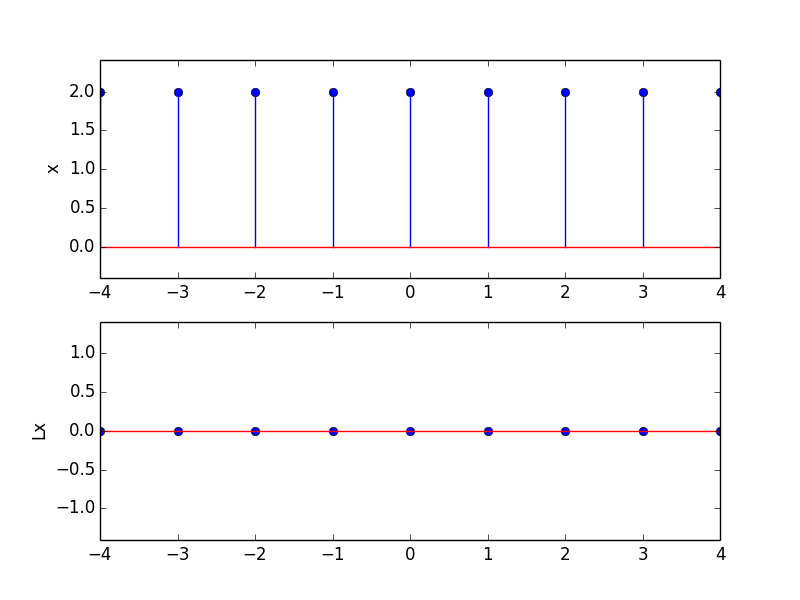
\includegraphics[width=\textwidth]{images/p2-1}
	\caption{$M=2, N=3, K=3$ ($x$ scale is $\pi$)}
	\label{fig:p2-1}
\end{figure}

\item Figure \ref{fig:p2-2} shows the results for$M=2, N=3, K=4$. After upsampling by 2 (second row), we need the cut-off frequency of $g$ to be $\frac{\pi}{4} \leq w_c \leq \frac{3\pi}{4}$. After apply downsampling by 3 (forth row), the gap is $\frac{\pi}{2}$. Therefore the gap is reduced by a third after upsampling by 3 (fifth row). So the second condition for cut-off frequency is $\frac{\pi}{4} \leq w_c \leq \frac{5\pi}{12}$. 
\[\frac{\pi}{4} \leq w_c \leq \frac{3\pi}{4} \text{ and } \frac{\pi}{4} \leq w_c \leq \frac{5\pi}{12} \Rightarrow \frac{\pi}{4} \leq w_c \leq \frac{5\pi}{12}\]
\begin{figure}
	\centering
	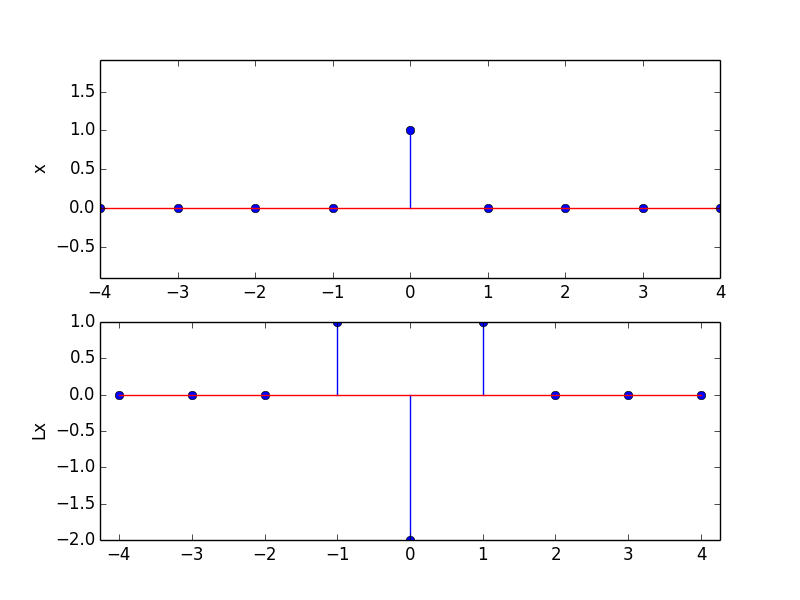
\includegraphics[width=\textwidth]{images/p2-2}
	\caption{$M=2, N=3, K=4$ ($x$ scale is $\pi$)}
	\label{fig:p2-2}
\end{figure}

\item If the signal in $[-\frac{2\pi}{K},\frac{2\pi}{K}]$, the gap's width is 
\[2\pi - \frac{2\pi}{K} -\frac{2\pi}{K} = 2\pi(1-\frac{2}{K})\]
After upsampling by $M$, the range is $[-\frac{2\pi}{KM},\frac{2\pi}{KM}]$ and the gap is $\frac{2\pi}{M} (1-\frac{2}{K})$. Therefore the first condition of $w_c$ is 
\[\frac{2\pi}{KM} \leq w_c \leq \frac{2\pi}{KM} + \frac{2\pi}{M} (1-\frac{2}{K}) \Leftrightarrow \frac{2\pi}{KM} \leq w_c \leq \frac{2\pi}{M} (1-\frac{1}{K})\]
After downsampling by $N$, the $[-\frac{2\pi N}{KM},\frac{2\pi N}{KM}]$ and the gap is $2\pi - \frac{2\pi N}{KM} - \frac{2\pi N}{KM} = 2\pi(1-\frac{2}{KM})$. So the second condition of $w_c$ is
\[ \frac{2\pi N}{KM} \leq w_c \leq \frac{2\pi N}{KM} + 2\pi(1-\frac{2}{KM}) \Leftrightarrow \frac{2\pi N}{KM} \leq w_c \leq 2\pi(\frac{1}{N} - \frac{1}{KM}) \]
Combining the first and second condition gives
\[ \frac{2\pi}{KM} \leq w_c \leq 2\pi(\frac{1}{N} - \frac{1}{KM}) \qquad (\because M<N\text{ so the second condition is tighter})\]
\end{enumerate}
	\section{Adaptive Filter and LMS}\label{sec:p3}

\begin{enumerate}[(a)]
\item We are given the model $\Expect{x[0]x[m]} = 2^{-\abs{m}} + 4^{-\abs{m}} = a_x[m]$, therefore we can use probabilistic cost function for this problem.
\[C(w) = \gamma_d - 2w^\top R_{xd} + w^\top R_x w\]

\item 
\begin{align*}
	R_x
	&= \Expect{X[n] X[n]^\top} \\
	&= \vect{
		a_x[0] & a_x[1] & a_x[2] & \cdots & a_x[L-1] \\
		a_x[1] & a_x[0] & a_x[1] & \cdots & a_x[L-2] \\
		a_x[2] & a_x[1] & a_x[0] & \cdots & a_x[L-3] \\
		\vdots & \vdots & \vdots & \ddots & \vdots \\
		a_x[L-1] & a_x[L-2] & a_x[L-3] & \cdots & a_x[0]
		}
\end{align*}

For $L \geq 3$,

For $L = 2$

For $L = 1$

\item

\item 
\end{enumerate}
	\section{Signal Sets and Spaces}\label{sec:part4}
	\section{Ideal-Matched Sampling and Interpolation with Nonorthogonal Filters}\label{sec:p5}
	\section{Python: Interpolation Games}\label{sec:p6}

For $\phi_2$, we consider the equation $1/(z/8 + 3z/4 +z^{-1}/8)$:
\begin{align*}
	\frac{1}{\frac{1}{8}z + \frac{3}{4} + \frac{1}{8}z^{-1}}
	&= \frac{8}{z + 6 + z^-1} \\
	&= \frac{8}{z^{-1}(z^2 + 6z + 1)} \\
	&= \frac{8}{z^{-1}(z+3+2\sqrt{2})(z+3-2\sqrt{2})} \\
	&= \frac{8}{(1+(3+2\sqrt{2})z^{-1})(z+3-2\sqrt{2})} \\
	&= \frac{\frac{8}{3+2\sqrt{2}}}{(z^{-1}+3-2\sqrt{2})(z+3-2\sqrt{2})} \\
	&= \frac{\sqrt{\frac{8}{3+2\sqrt{2}}}}{z^{-1}+3-2\sqrt{2}} \cdot \frac{\sqrt{\frac{8}{3+2\sqrt{2}}}}{z+3-2\sqrt{2}}
\end{align*}
Therefore, we can choose $\mu = \sqrt{\frac{8}{3+2\sqrt{2}}}$ and $\gamma = 2\sqrt{2}-3$.

Figure \ref{fig:p6b} shows the interpolation results on the UIN and Figure \ref{fig:p6b} shows the results on 5 points inputted by mouse. The results of $\phi_0, \phi_1$, and $\phi_3$ are the same for the second figure.
\begin{figure}[htbp]
	\centering
	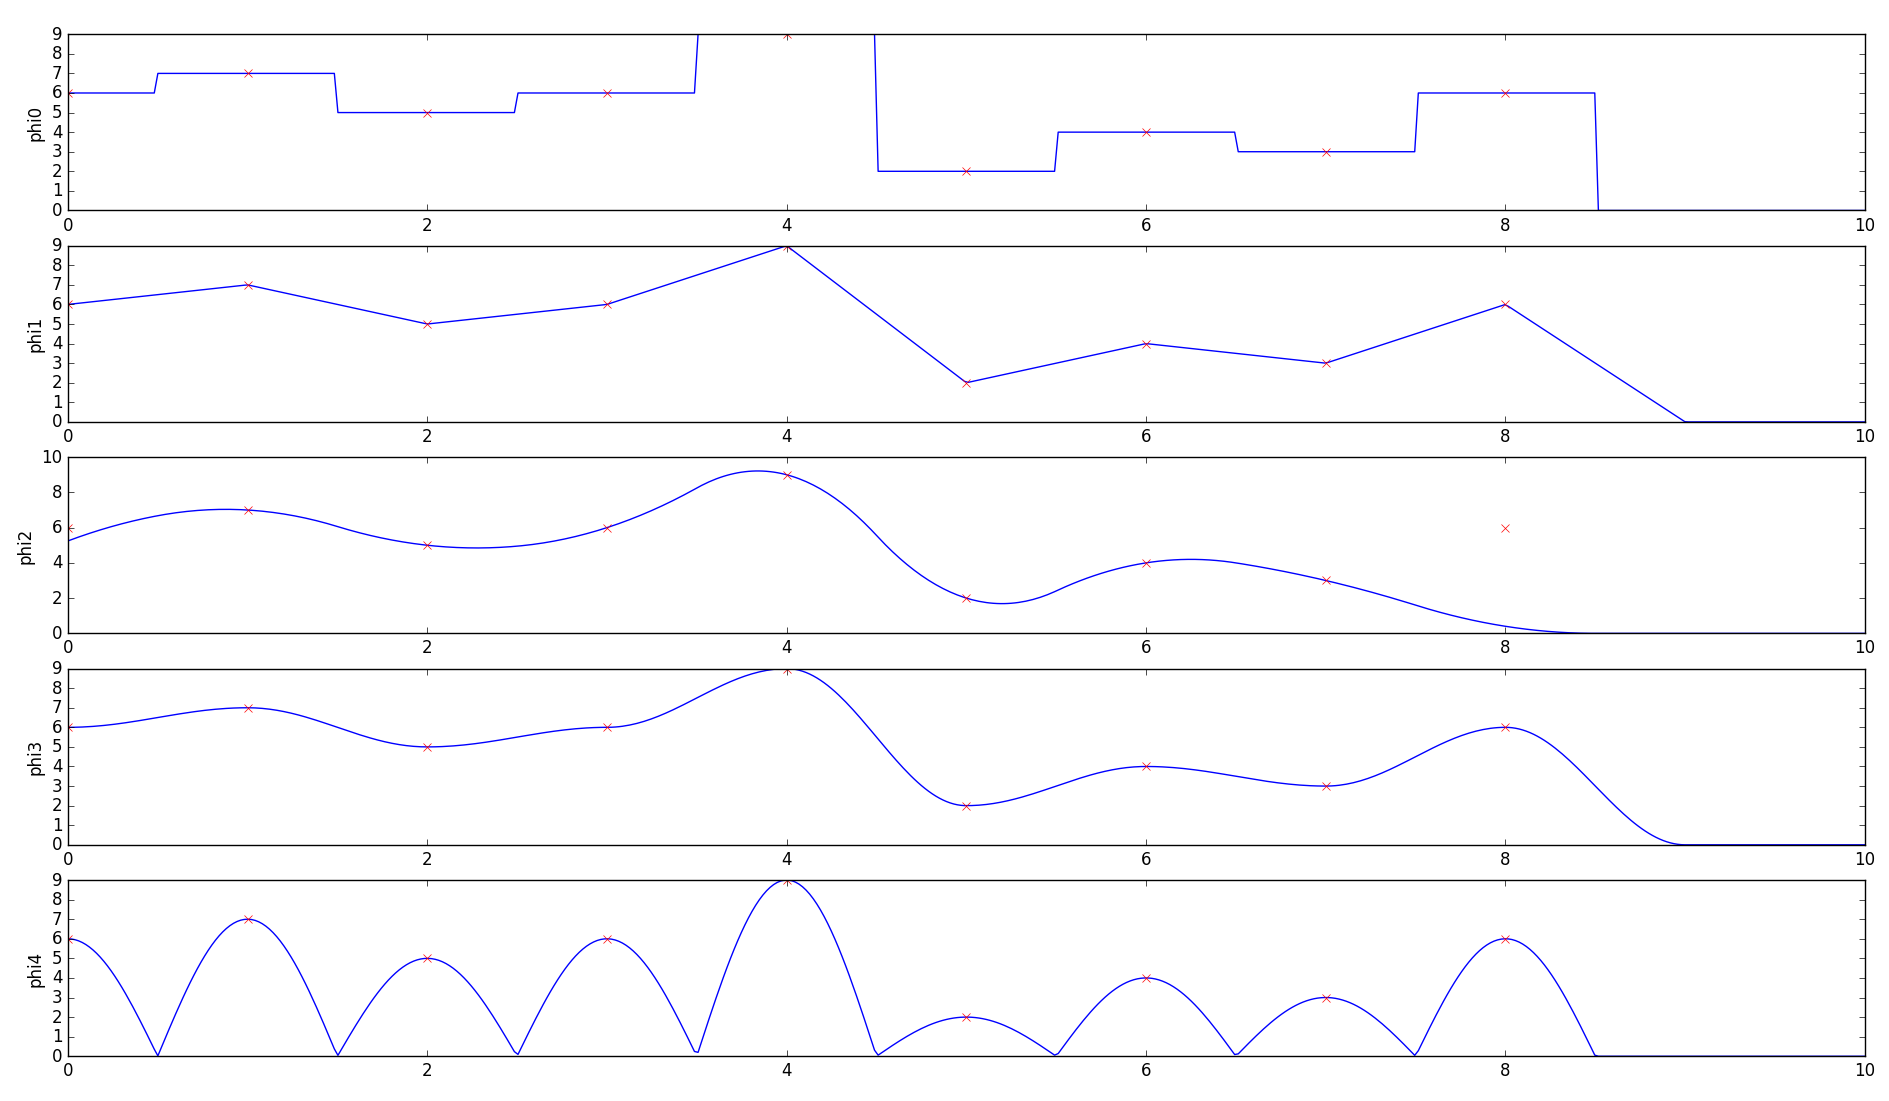
\includegraphics[width=\linewidth]{images/p6b}
	\caption{Interpolation results on the UIN}
	\label{fig:p6b}
\end{figure}

\begin{figure}[htbp]
	\centering
	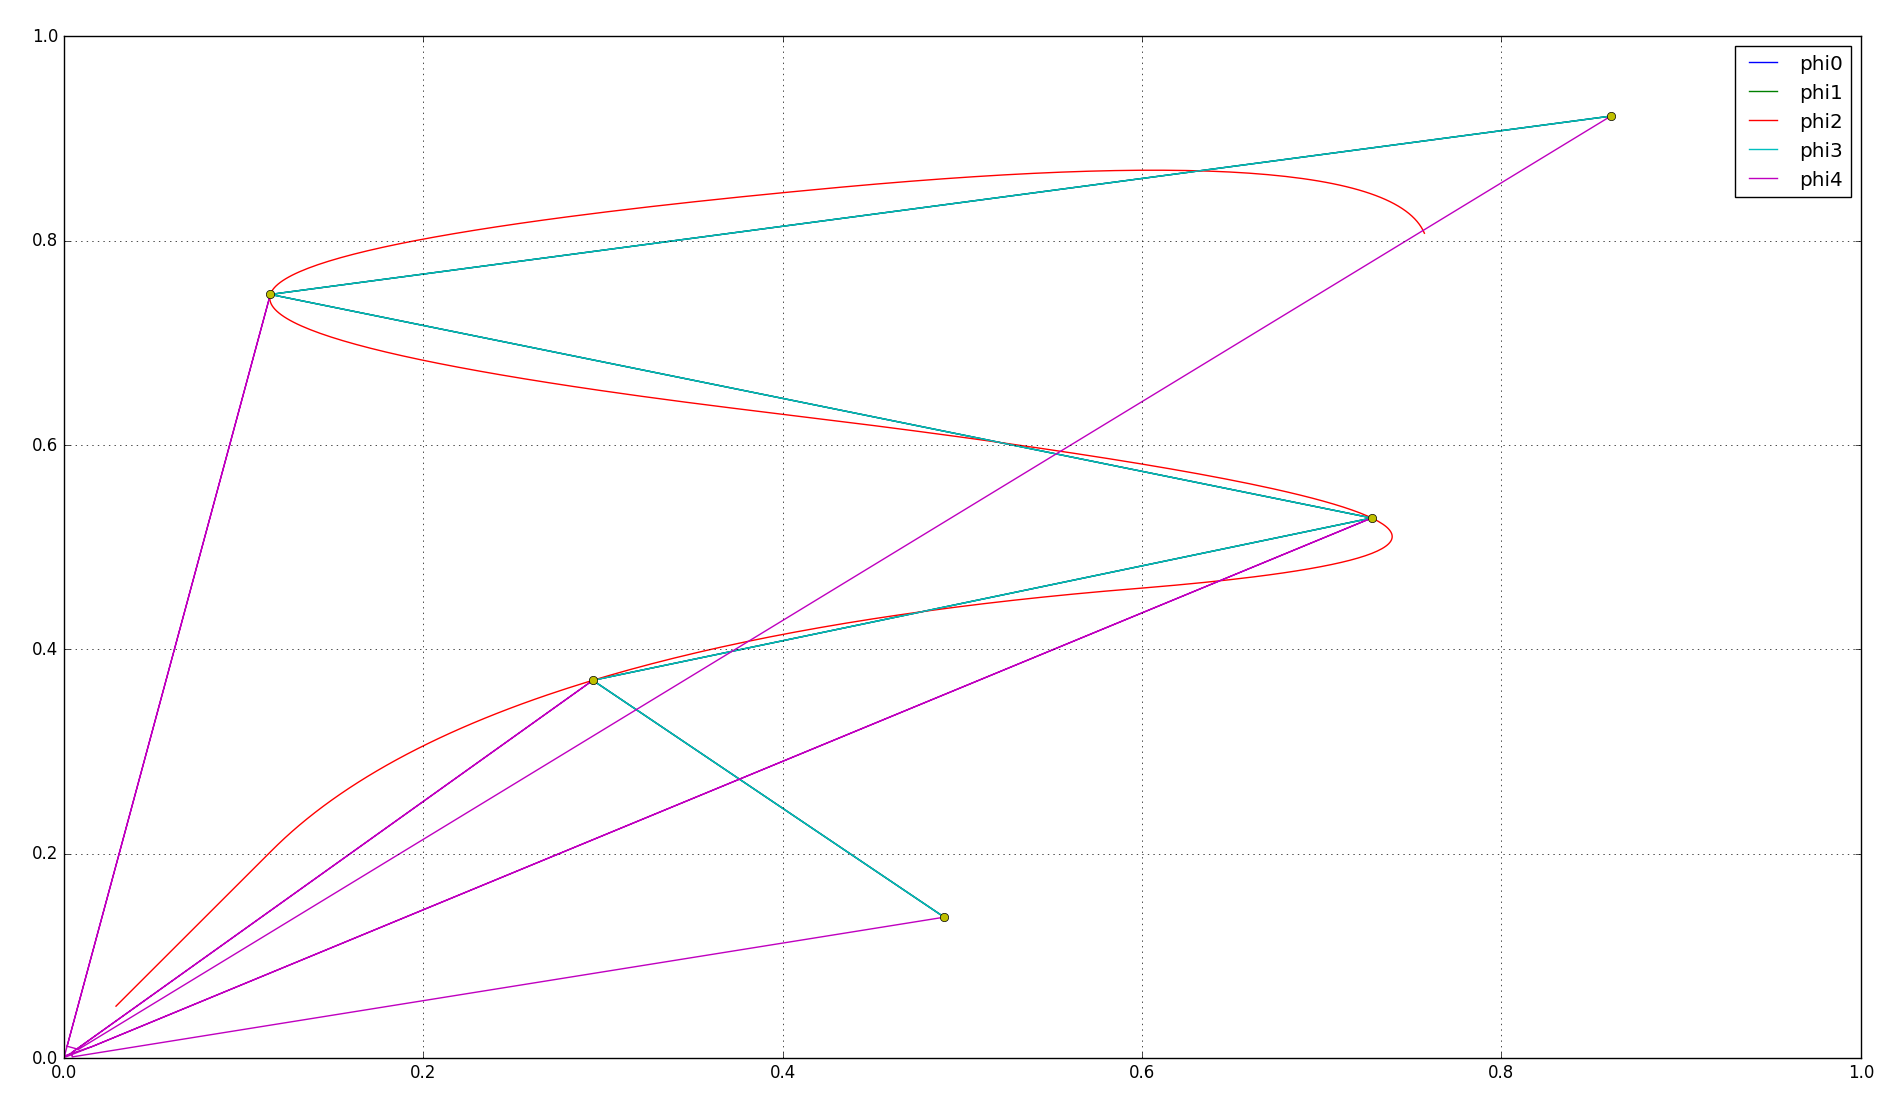
\includegraphics[width=\linewidth]{images/p6c}
	\caption{Interpolation results on 5 inputted points}
	\label{fig:p6c}
\end{figure}
	\section{Python Exercise: Image Scaling with Separable Filters}\label{sec:p7}

Figure \ref{fig:p7} shows the results of the four pre-filters. Since the visual difference is subtle, their corresponding MSEs are included. Method (a) and (c) are actually the same since $h = \delta$ so their MSEs are the same. The pattern (around leg and scarf area) of method (b) is overly smoothed.

\begin{figure}[htbp]
	\centering
	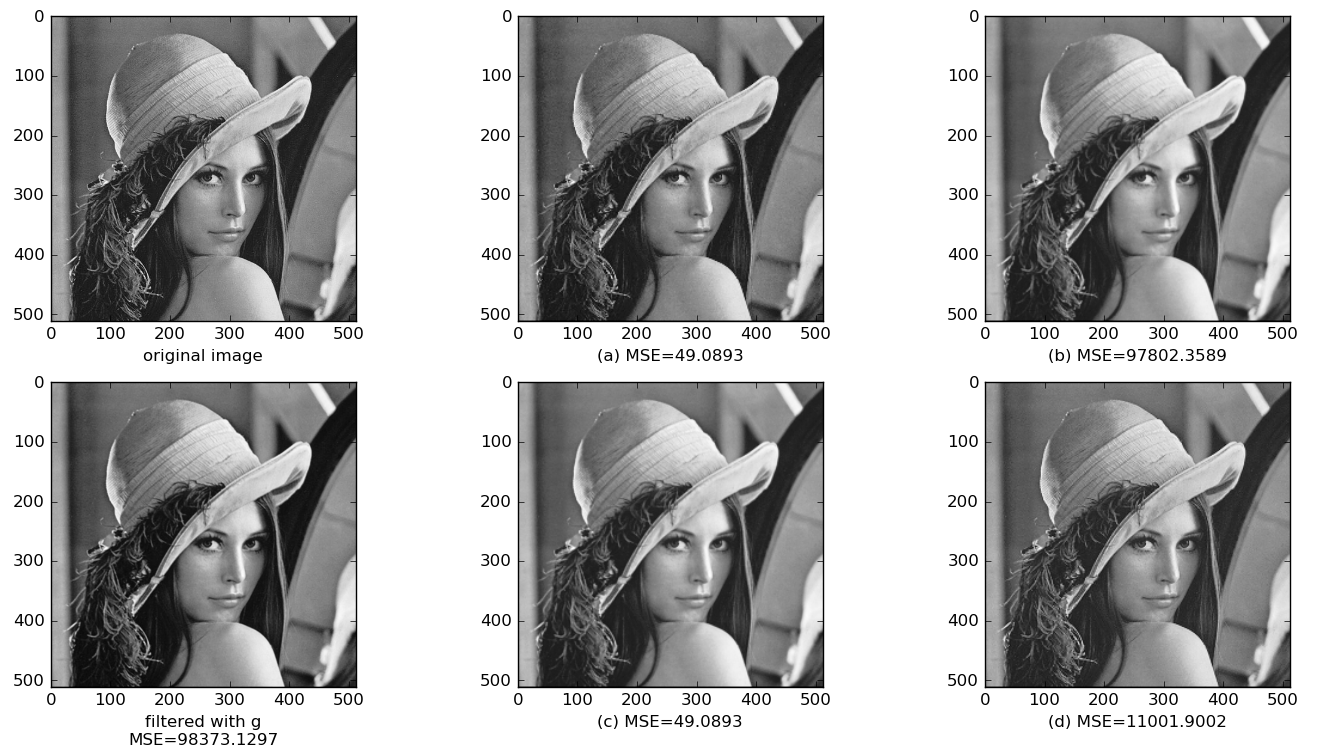
\includegraphics[width=\textwidth]{images/p7}
	\caption{Original image and four pre-filters (a-d) with corresponding MSE}
	\label{fig:p7}
\end{figure}
	\section{Python Exercise: Two-Channel Delay Recovery}\label{sec:p8}

\begin{figure}[htbp]
	\centering
	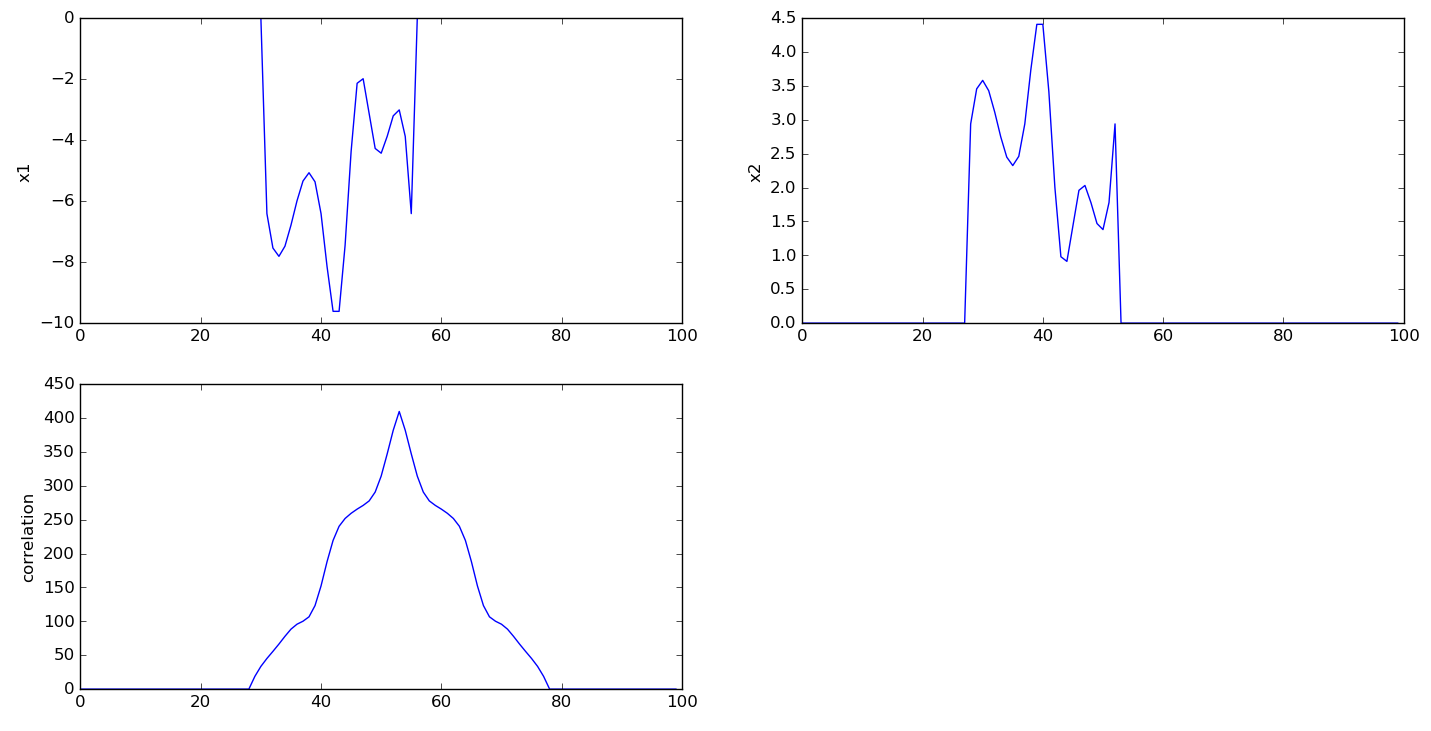
\includegraphics[width=\textwidth]{images/p8-1}
	\caption{An output of two-channel delay recovery. The top 2 images are $x_1$ and $x_2$, where the third one is their cross-correlation.}
	\label{fig:p8-1}
\end{figure}

Figure \ref{fig:p8-1} shows an the generated signals and their cross-correlation. The output of the code is:

\begin{lstlisting}
delta=-3, rho=-2.1807
n2=27, n1=30, n2-n1=-3
alpha1=-1.0682, alpha2=0.4899, alpha1/alpha2=-2.1807
\end{lstlisting}
	\section{Python Exercise: Multirate Systems}\label{sec:p9}

\begin{figure}[htbp]
	\centering
	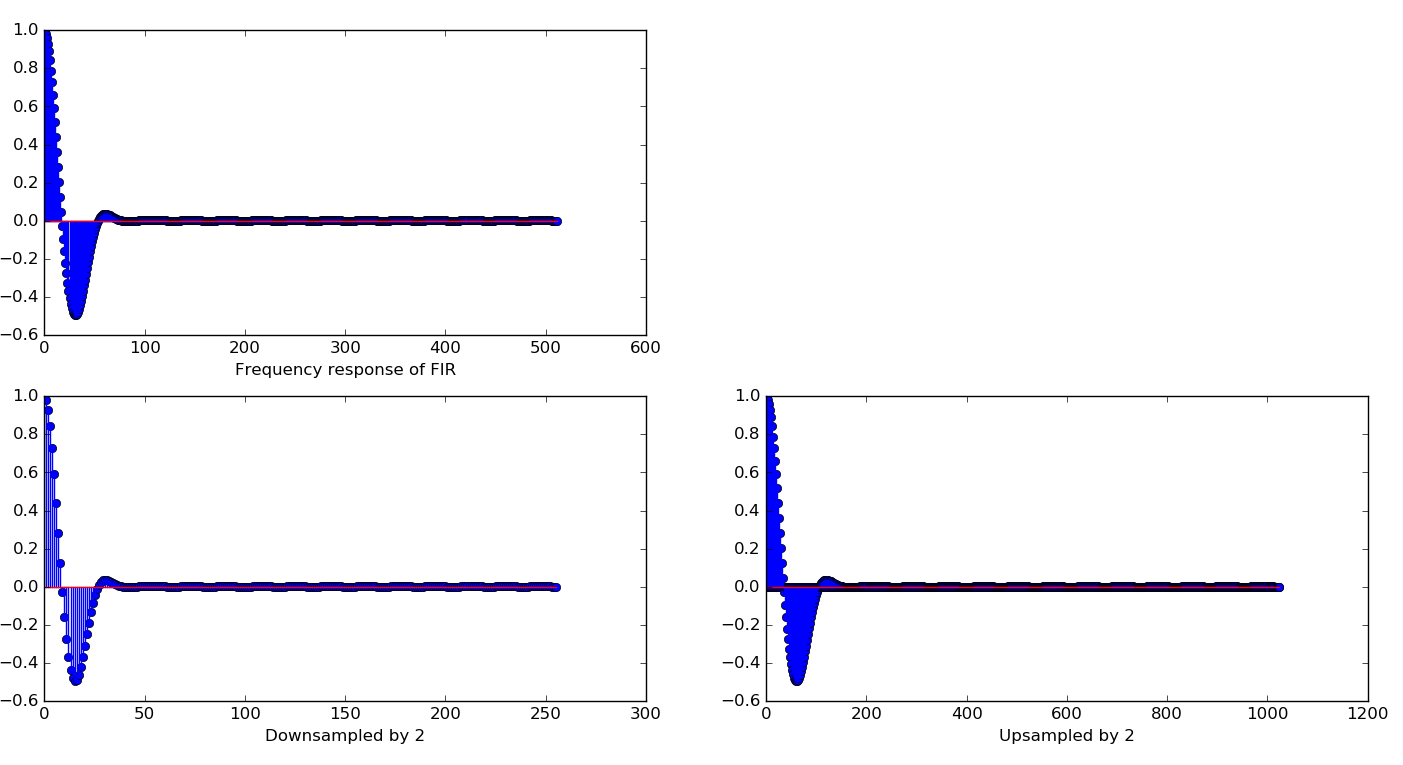
\includegraphics[width=\textwidth]{images/p9-1}
	\caption{An output of generated FIR filter (frequency response).}
	\label{fig:p9-1}
\end{figure}

\begin{figure}[htbp]
	\centering
	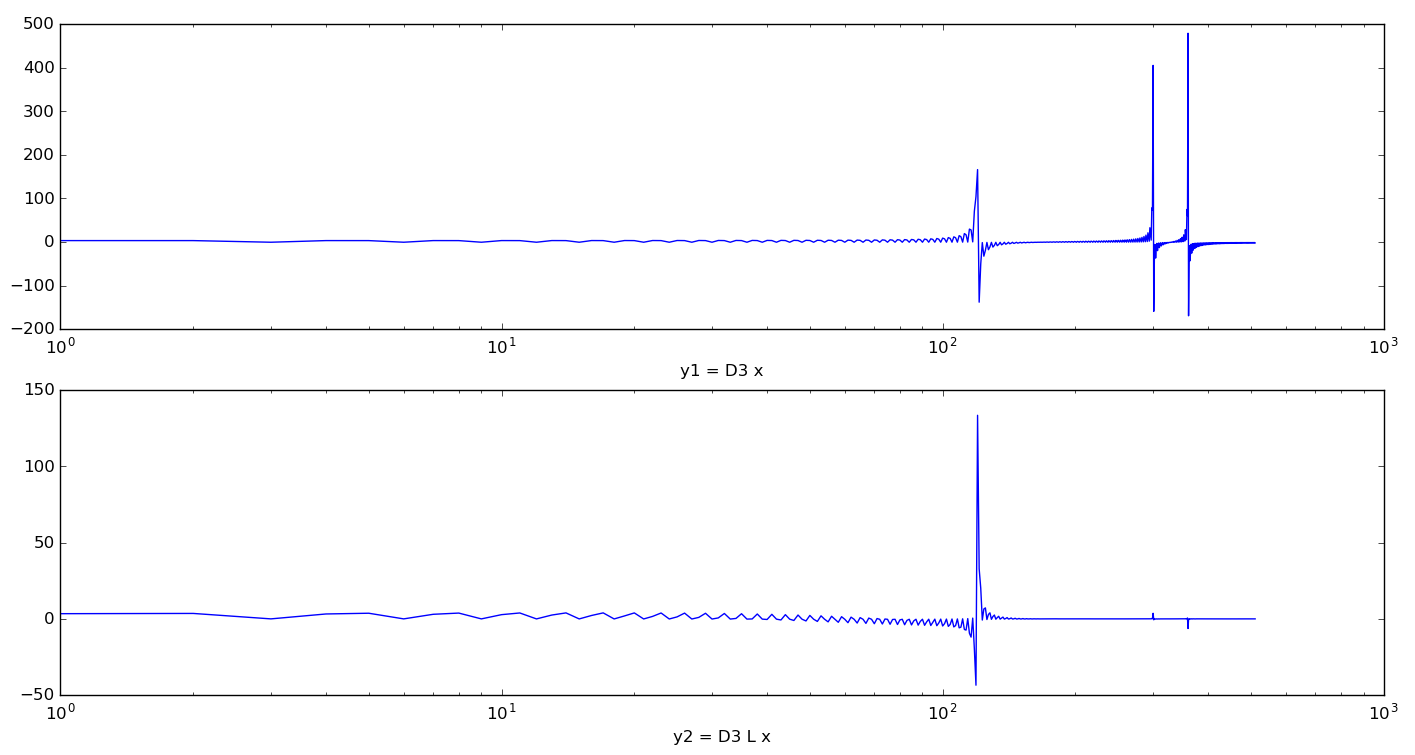
\includegraphics[width=\textwidth]{images/p9-2}
	\caption{An output of $y_1 = D_3 x$ (top) and $y_2 = D_3 L x$ (bottom) (frequency response, in log-scale).}
	\label{fig:p9-2}
\end{figure}

Figure \ref{fig:p9-1} shows the frequency response of FIR lowpass filter (with sample rate of 100). Although the plots look similar due to scaling, the number of samples differs, i.e. downsampled version has half the amount and upsampled version has twice the amount of samples as the original one.

Figure \ref{fig:p9-2}  shows the frequency response of $y_1$ and $y_2$ in log-scale. It is obvious that $y_1$ suffers the aliasing effects (2 spikes towards the end) while that effect on $y_2$ is not significant.

\end{document}